\section{Market Analysis}
  \label{blMAanalysis}
Market analysis determines the main potential users and is mainly dependent on the quality and quantity of the obtained data. There are four types of the measurement data sets and it is convenient to analyze them separately. Figure \ref{MA} on page \pageref{MA} gives the market diagram with the different data sets.
\begin{figure} [ht]
	\begin{center}
 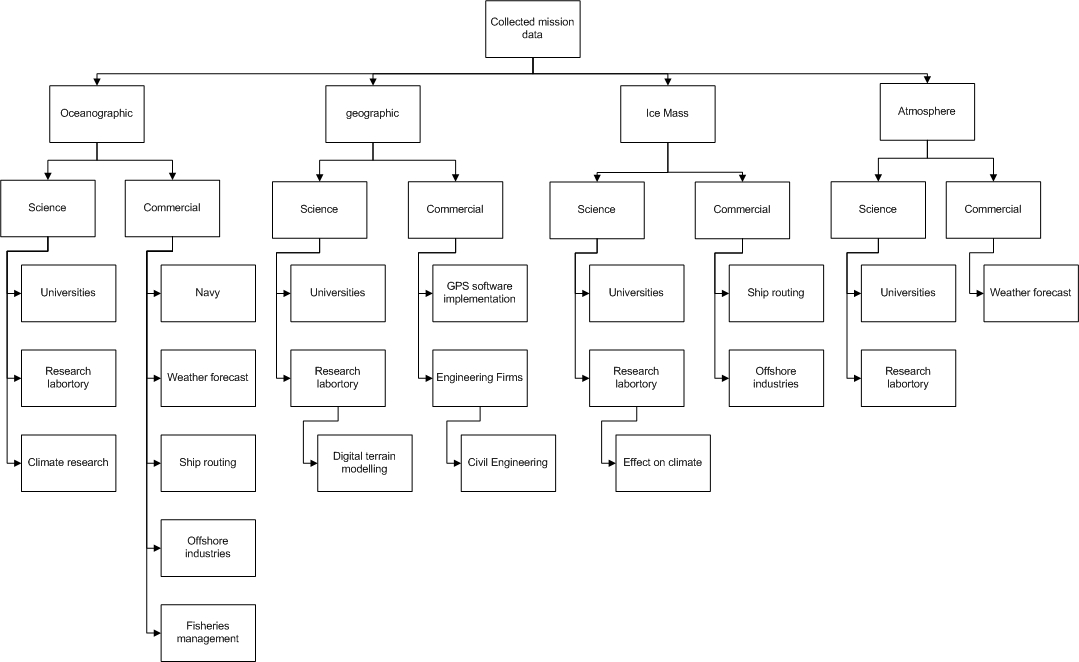
\includegraphics[width=0.85\textwidth,angle=0]{chapters/img/Market_analysis.jpg}	
	\caption{Market Breakdown Diagram with different data sets \cite{Market}}
	\label{MA}
	\end{center}
\end{figure}


In the Market Breakdown Diagram, each data type has both science and commercial potential users. For example, in the science field the oceanographic data can be used for climate research. Scientists can study the evolution of weather patterns from the ocean system by modeling changes in the heat distribution of the ocean. On the other hand, in the commercial field maps of currents, eddies and vector winds are used in commercial shipping and recreational yachting to optimize routes. All the blocks in the diagram could be potential return on investment on short or long term.
